\documentclass[12pt]{report}
\usepackage{polski}
\usepackage[a4paper, margin=2.5cm]{geometry}
\usepackage{graphics}
\usepackage[export]{adjustbox}
\usepackage{float}
\usepackage{amsmath}
\usepackage{xcolor}
\usepackage{multirow}
\usepackage{array}


\title{Analiza wyników pomiarowych z prób spęczania z wykorzystaniem aplikacji komputerowej - praca inżynierska}
\date{12.01.2026}
\author{Szymon Miłkowski}

\begin{document}
	\maketitle
	\tableofcontents
	
	\chapter{Wstęp}
	\section{Czego dotyczy praca}
	\paragraph{}
	Praca obejmuje stworzenie aplikacji komputerowej do graficznej i komputerowej analizy wyników pomiarowych z prób spęczania.
	
	\section{Opis próby spęczania}
	\paragraph{}
	Próba spęczania polega na ściskaniu próbki wzdłuż jednej osi (pionowej) przez maszynę
	badawczą z zadaną prędkością. Podczas próby materiał odkształca się, zmniejszając swoją
	wysokość w kierunku działania siły oraz - zgodnie z zasadą zachowania objętości - zwiększając swoją szerokość w pozostałych kierunkach. Próby mogą być wykonywane w piecu oraz w temperaturze otoczenia - tzn. poza piecem.
	
	\paragraph{}
	Podczas tego procesu, materiał wewnątrz płynie, wypychając materiał na ścianach bocznych na zewnątrz, a materiał przy podstawach trze o górną i dolną ścianę maszyny, co
	hamuje jego przemieszczenie na zewnątrz. Efekt ten powoduje zaokrąglenie powierzchni bocznej próbki.
	
	\paragraph{}
	Wielkości mierzone przez maszynę, zawarte w pliku wyjściowym pomiaru to: czas, obciążenie, przesunięcie oraz zadany sygnał.
	
	\paragraph{}
	Po przeliczeniu wartości sił i przemieszczenia na zależność naprężenia od odkształcenia możliwe jest wyznaczenie modułu sprężystości, modułu plasytczności, granicy plastyczności, a także wytrzymałości na spęczanie.
	
	\paragraph{}
	Przeprowadzone spęczania w stanie stałociekłym pozwalają również na wyznaczenie wartości lepkości badanego materiału w funkcji prędkości ścinania. (wzory jutro) 
	
	\pagebreak
	\section{Opis maszyny pomiarowej}
	\paragraph{}
	
	\begin{figure}[H]
		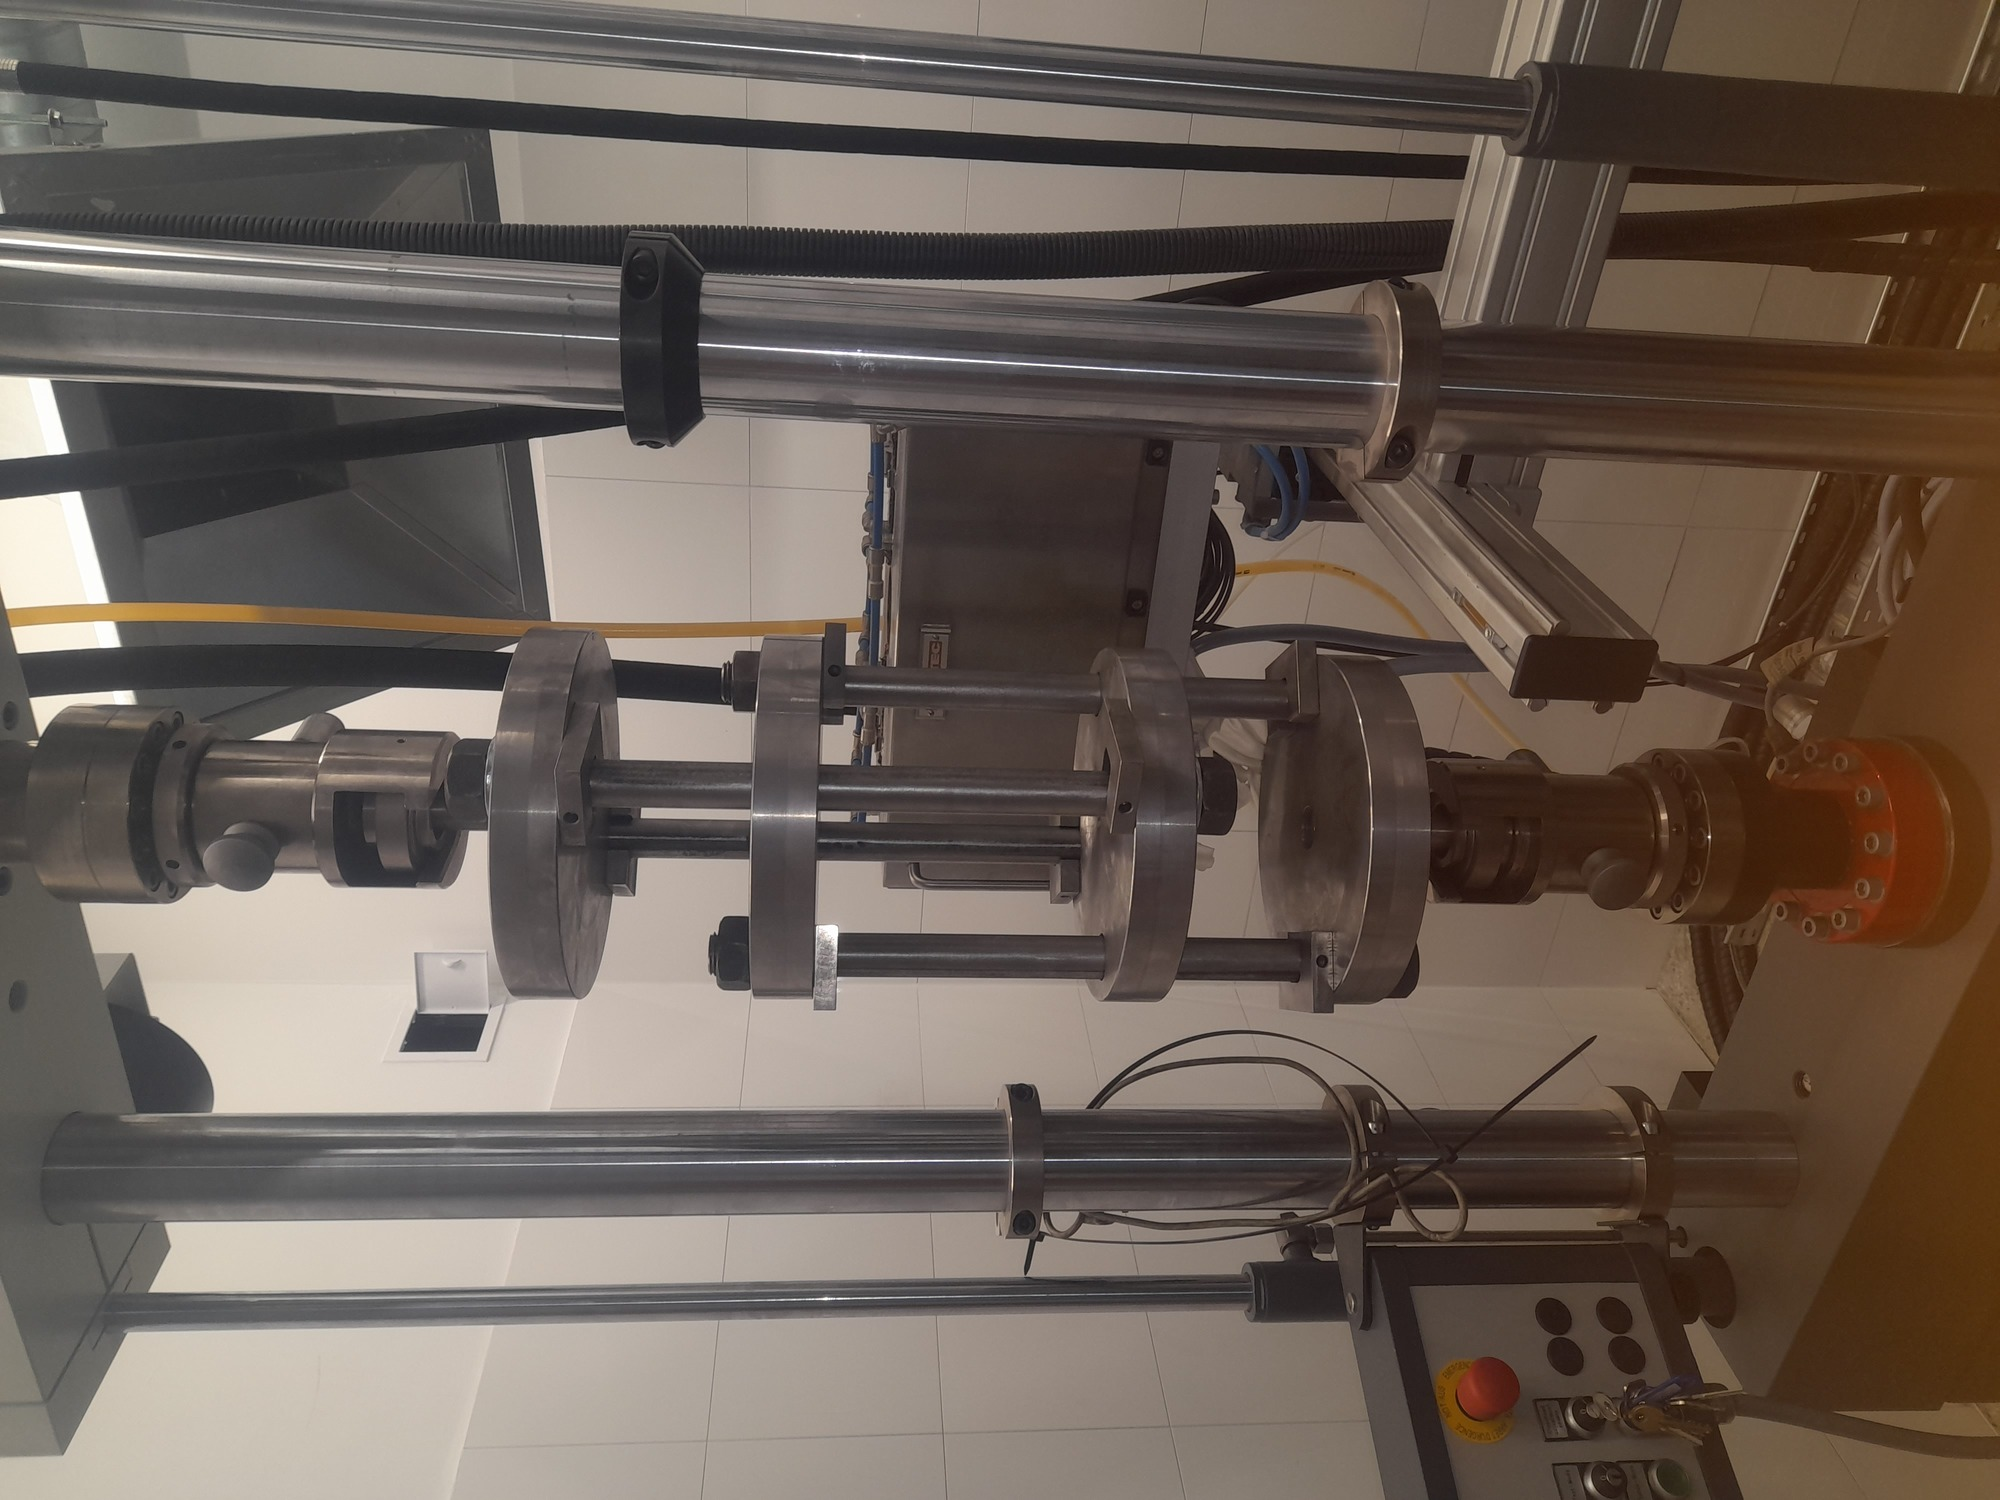
\includegraphics[width=.8\textwidth, angle=-90, center]{images/ZwickHB100a.jpg}
		\caption{Maszyna do przeprowadzania prób spęczania Zwick HB100}
	\end{figure}
	
	\section{Aktualne rozwiązania}
	\subsection{[nazwa programu]}
	\paragraph{}
	Program służy do wyświetlania danych na wykresie. Posiada opcje importu danych z formatu W01, zmiany osi i serii danych oraz eksportu do pliku tekstowego CSV. Program ten jednak jest trudniejszy w obsłudze oraz przydatne funkcjonalności wymagają repetytywnych czynności ze strony użytkownika.
	
	\section{Co zawiera praca}
	\paragraph{}
	Ten dokument zawiera opis problemu, cel i założenia, napotkane przeszkody, ogólną strukturę i sposób działania aplikacji oraz niektóre szczegóły implementacji.
	
	
	\chapter{Cel i teza pracy}
	\section{Cel}
	\paragraph{}
	Celem projektu jest stworzenie kompatybilnego i wydajnego programu, który usprawni
	pracę z wynikami pomiarowymi z prób spęczania. Główny nacisk kładziony jest na maksy-
	malną oszczędność czasu i szybkość w obsłudze dla wprawionego użytkownika, co można
	osiągnąć przez prosty i czytelny interfejs zoptymalizowany pod najczęściej wykonywane
	operacje. Program wykonany w pracy ma na celu obróbkę danych pomiarowych wygenerowanych przez maszynę wytrzymałościową Zwick HB100. Surowe wyniki pomiarów zawierają wartości sił zarejestrowanych dla pozycji siłownika maszyny. W celu wyznaczenia właściwości badanego materiału dane te muszą zostać przeliczone na zależność naprężenia od odkształcenia badanej próbki. Maszyna posiada aplikację do przeglądania wyników prób oraz ich obróbki, niemniej jednak obsługa tego programu jest czasochłonna i nieintuicyjna. Zaplanowane w pracy inżynierskiej oprogramowanie ma na celu istotne skrócenie obróbki danych pomiarowych realizowane przy pomocy interaktywnych wykresów, umożliwiających jednoczesną obserwację kształtu zarejestrowanych zależności.
	
	\paragraph{}
	Dodatkowym celem jest również wysoka kompatybilność programu zarówno z nowymi
	jak i starszymi systemami operacyjnymi oraz wysoka wydajność nawet na starym sprzęcie
	komputerowym.
	
	\section{Teza}
	Stwierdzono brak powszechnego występowania prostych i darmowych aplikacji umożliwiających obróbkę danych pomiarowych z wykorzystaniem interaktywnych wykresów. W związku z powyższym sformułowano tezę, że analiza wyników pomiarowych jest możliwa dzięki takiemu podejściu, co wykazano w niniejszej pracy.
	
	\chapter{Opis narzędzi wykorzystanych do realizacji pracy}
	\section{Język programowania}
	\paragraph{}
	Wybranym językiem programowania do stworzenia aplikacji został \textbf{język C} w standardzie C11. Cechuje się on bardzo wysoką kontrolą nad działaniem programu, co pozytywnie wpływa na wydajność oraz minimalną ilością zależności, dzięki czemu łatwiej zachować kompatybilność z większą ilością systemów. Narzędzia do pracy z C pozwalają na stworzenie statycznego pliku wykonywalnego, który nie będzie potrzebować procesu instalacji.
	
	\section{Środowisko graficzne}
	\paragraph{}
	Do obsługi grafiki oraz urządzeń wejścia (mysz i klawiatura) została wykorzystana \textbf{biblioteka Raylib}, posiadająca łatwe w obsłudze, bogate API kompatybilne z wieloma systemami operacyjnymi. Raylib nie posiada nie posiada zależności, można ją dołączyć statycznie do pliku wykonywalnego i wymaga jedynie obsługi OpenGL w sterowniku graficznym.
	
	\section{Kompilacja}
	\paragraph{}
	Prace programistyczne odbywały się na systemach Linux oraz MacOS (ARM), gdzie użyto domyślnych dla systemu kompilatorów C - odpowiednio GCC oraz Clang. Kompilacja na system Windows odbywała się na systemie Linux z wykorzystaniem MinGW. Projekt używa CMake do zarządania kompilacją.
	
	
	\chapter{Opis utworzonej aplikacji}
	\section{Architektura aplikacji}
	\subsection{Ogólna struktura aplikacji}
	\subsubsection{Komponenty}
	Interfejs graficzny aplikacji podzielony jest na "komponenty" - funkcje zawierające logikę kontrolną oraz rysujące pewien element interfejsu. Wywołanie tej funkcji oznacza, że komponent istnieje w obecnej klatce.
	Funkcje te mogą wywoływać inne funkcje komponentów, co tworzy swego rodzaju strukturę drzewa komponentów, rozpoczynającą się w głównej pętli programu. Pozycja w strukturze drzewa nie ma jednak wpływu na rozmieszczenie elementu, pozycja jest statyczna, lub określana poprzez podane parametry.
	
	\subsubsection{Zarządzanie stanem}
	Inspirowane działaniem innego drzewiastego systemu komponentów graficznych - webowym Reactem - komponenty, jeśli to konieczne, operują na dwóch rodzajach danych: właściwości (\textit{props}) i stan (\textit{state}).
	\paragraph{Właściwości} są podawane do funkcji komponentu jako kopia (pass by value), bądź stały wskaźnik, mają za zadanie sterować zachowaniem i wyglądem komponentu.
	\paragraph{Stan} jest podawany jako wskaźnik do pamięci zarządzanej przez rodzica (komponent wywołujuący), ma za zadanie przechowywanie stanu komponentu między wywołaniami, jest modyfikowany głównie przez sam komponent oraz jego dzieci (jeśli zostanie podany do nich jako ich stan).
	\paragraph{Stan globalny} jest wykorzystywany w niektórych komponentach, które z założenia mają istnieć tylko w jednej sztuce jednocześnie, jak lista otwartych plików lub narzędzia diagnostyczne \verb|FPSCounter| i \verb|Clock|, jako zmienne globalne w jednostce translacyjnej (niewidoczna poza obecnym plikiem .c), lub statyczne zmienne lokalne w funkcji komponentu.
	
	
	\pagebreak
	\subsection{Rysowanie wykresu}
	Jako podstawa rysowania wykresu, została wykorzystana funkcja Rzylib \verb|DrawSplineLinear|, łącząca podane współrzędne pikseli prostymi odcinkami. To wydajny sposób narysowania wielu prostych jednocześnie, co przy wystarczającej gęstości punktów daje iluzję krzywej.
	
	\begin{verbatim}
		DrawSplineLinear(state->point_buffer, state->visible.count, 2.f, DARKBLUE);
	\end{verbatim}
	
	\subsubsection{Poruszanie się w widoku}
	Aby zwiększyć interaktywność, użytkownik może się poruszać po płaszczyźnie XY, przeciągając płaszczyznę myszką, oraz przybliżając i oddalając kółkiem myszy. Manipulowane są w ten sposób zmienne skali oraz przesunięcia uwzględnione w przekształceniu punktów ze współrzędnych kartezjańskich na współrzędne ekranu.
	
	\subsubsection{Transformacja współrzędnych}
	
	Punkt podlega przekształceniu liniowemu:
	
	\begin{equation}
		x = \frac{z(x_p - x_v) - x_{S}}{x_{E} - x_{S}} * W + x_O
	\end{equation}
	gdzie \\
	$z$ - współczynnik skali \\
	$x_p$ - współrzędna $x$ punktu w układzie kartezjańskim \\
	$x_v$ - przesunięcie $x$ w układzie kartezjańskim \\
	$x_S$ - współrzędna $x$ lewej krawędzi układu kartezjańskiego przy zerowym przesunięciu \\
	$x_E$ - współrzędna $x$ prawej krawędzi układu kartezjańskiego przy zerowym przesunięciu \\
	$W$ - szerokość wykresu w pikselach \\
	$x_O$ - odległość prawej krawędzi wykresu od prawej krawędzi ekranu
	\\\\
	
	\begin{equation}
		y = \frac{-z(y_p + y_v) - y_{S}}{y_{E} - y_{S}} * H + y_O
	\end{equation}
	gdzie \\
	$z$ - współczynnik skali \\
	$y_p$ - współrzędna $y$ punktu w układzie kartezjańskim \\
	$y_v$ - przesunięcie $y$ w układzie kartezjańskim \\
	$y_S$ - współrzędna $y$ dolnej krawędzi układu kartezjańskiego przy zerowym przesunięciu \\
	$y_E$ - współrzędna $y$ górnej krawędzi układu kartezjańskiego przy zerowym przesunięciu \\
	$H$ - wysokość wykresu w pikselach \\
	$y_O$ - odległość górnej krawędzi wykresu od górnej krawędzi ekranu \\
	
	Zmiana znaku $y_p$ jest spowodowana, tym że oś +Y we współrzędnych ekranowych skierowana jest w dół.
	
	\pagebreak
	\paragraph{Implementacja}
	W kodzie programu zaimplementowane jest to dwuetapowo.
	\paragraph{Obliczanie granic widocznego fragmentu}
	\begin{verbatim}
		Bounds compute_bounds(const float zoom, const Vector2 pan) {
			return (Bounds) {
				.start_x = PLOT_START_X / zoom + pan.x,
				.end_x = PLOT_END_X / zoom + pan.x,
				.start_y = PLOT_START_Y / zoom / ((float) PLOT_WIDTH / PLOT_HEIGHT) + pan.y,
				.end_y = PLOT_END_Y / zoom / ((float) PLOT_WIDTH / PLOT_HEIGHT) + pan.y,
			};
		}
	\end{verbatim}
	
	\paragraph{Transformacja pojedynczego punktu}
	\begin{verbatim}
		Vector2 transform_v_to_pixel(const Vector2 v, const Bounds bounds) {
			return (Vector2){
				.x = (v.x - bounds.start_x)
					/ (bounds.end_x - bounds.start_x)
					* PLOT_WIDTH + PLOT_OFFSET_X,
					
				.y = (-v.y - bounds.start_y)
					/ (bounds.end_y - bounds.start_y)
					* PLOT_HEIGHT + PLOT_OFFSET_Y,
			};
		}
	\end{verbatim}
	
	\paragraph{Transformacja wielu punktów jednocześnie} jest zoptymalizowana pod kątem ilości niepotrzebnych operacji.
	
	\pagebreak
	\subsection{Minimalizacja renderowanych punktów}
	\subsubsection{Opis problemu}
	Podczas przegladania wykresu, nie każdy punkt będzie widoczny jednocześnie. Chcąc zminimalizować ilość punktów podlegających transformacji oraz rysowaniu, należy znaleźć zakres punktów widocznych na ekranie.
	
	\subsubsection{Szukanie pierwszego punktu}
	Zakładając, że współrzędna $x$ w zestawie danych jest niemalejąca, możemy potraktować zbiór $X$ jako posortowany zbiór danych i użyć wydajnego algorytmu \textbf{wyszukiwania binarnego}, o złożoności obliczeniowej $O(\log_2n)$.
	
	\begin{verbatim}
		int find_first_visible(const Vector2* data, const int count, const float start_x) {
			if (data[count - 1].x < start_x) return -1;
			
			int a = 0, b = count - 1;
			while (b - a > 1) {
				const int mid = (a + b) / 2;
				if (data[mid].x > start_x) b = mid;
				else a = mid;
			}
			return a;
		}
	\end{verbatim}
	
	\subsubsection{Transformacja punktów}
	Po znalezieniu pierwszego elementu zbioru wyjściowego, współrzędne są przekształcane i zapisywane w tablicy wyjściwej aż do napotkania punktu znajdującego się za prawą krawędzią widoku lub końca tablicy wejściowej. Wyszukiwanie binarne nie ma tutaj zastosowania, ponieważ i tak każdy widoczny punkt musi zostać przekształcony, co wiąże się z liniowym algorytmem.
	
	\begin{verbatim}
		VisiblePointsInfo compute_visible_points_offset(
		const DataSource data_source, Vector2* point_buffer, const Bounds bounds, const Vector2 offset
		) {
			VisiblePointsInfo res = {
				.start = find_first_visible(data_source.data, data_source.count, bounds.start_x - offset.x)
			};
			if (res.start == -1) return res;
			
			const float x_factor =  1 / (bounds.end_x - bounds.start_x) * PLOT_WIDTH;
			const float y_factor = -1 / (bounds.end_y - bounds.start_y) * PLOT_HEIGHT;
			
			const int visible_count = data_source.count - res.start;
			for (int i = 0; i < visible_count; i++) {
				const int i_source = i + res.start;
				point_buffer[i].x = (data_source.data[i_source].x - bounds.start_x + offset.x)
				* x_factor + PLOT_OFFSET_X;
				point_buffer[i].y = (data_source.data[i_source].y + bounds.start_y - offset.y)
				* y_factor + PLOT_OFFSET_Y;
				if (data_source.data[i_source].x > bounds.end_x - offset.x) {
					res.count = i + 1;
					return res;
				}
			}
			res.count = visible_count;
			return res;
		}
	\end{verbatim}
	Algorytm nie używa funkcji do transformacji pojedynczego punktu, co pozwala na obliczenie niezmiennych współczynników poza pętlą, unikając zbędnych operacji.
	
	\subsection{Wykrywanie zmian}
	\paragraph{}
	Transformacja wszystkich widocznych punktów jest mimo wszystko kosztowną operacją, dlatego wykonywana jest jedynie gdy reprezentacja punktów na wykresie powinna ulec zmianie. Odpowiada za to zmienna \textit{change}, zawierająca flagi sterujące rekalkulacją elementów wykresu, ustawiana przez funkcję odpowiadającą za obsługę wejścia.
	
	
	\section{Instrukcja opsługi}
	\subsection{Wczytywanie plików}
	\paragraph{}
	Wczytanie odbywa się poprzez upuszczenie jednego lub wielu plików na okno otwartego programu. Program jest w stanie wczytać dwa rodzaje plików.
	
	\subsubsection{Plik binarny W01}
	\paragraph{}
	Jest to plik produkowany przez oprogramowanie maszyny Zwick HB100 i zawiera serie danych z pomiaru. Dokładny opis formatu tego pliku znajduje się w sekcji 4.3.
	\paragraph{}
	Podczas wczytywania tego pliku, użytkownik jest pytany o wybranie kolumn odpowiadającym osiom X i Y.
	
	\subsubsection{Plik tekstowy CSV}
	Wykres wyeksportowany do pliku CSV, może zostać otwarty ponownie w aplikacji.
	
	\subsection{Obróbka wykresu}
	Po załadowaniu wykresu, do dyspozycji użytkownika są dostępne następujące operacje:
	
	\subsubsection{Przesuwanie (translacja)}
	Trzymając klawisz Lewy Ctrl i lewy przycisk myszy, wykres przesuwany jest zgodnie z ruchem kursora myszy. Podczas przesuwania pojawi się "cień" wykresu, odpowiadający miejscu w którym będzie znajdował się wykres po przesunięciu. Puszczenie leweko przycisku myszy zatwierdza przesunięcie, a puszczenie klawisza Lewy Ctrl anuluje przesunięcie.
	
	\subsubsection{Blokada przesuwania}
	Przyciski "Blokj X" i "Blokuj Y" blokują możliwość przesuwania wykresu wzdłuż danej osi. Jest to pomocna funkcja, jeśli użytkownik potrzebuje zmienić jedną współrzędną punktów.
	
	\subsubsection{Przesuwanie do zera}
	Przycisk "Zeruj start" przesuwa cały wykres tak, aby pierwszy punkt znajdował się w punkcie (0,0).
	
	\subsubsection{Odbicie}
	Przyciski "Odwróć X" i "Odwróć Y" odbijają daną współrzędną każdego z punktów względem zera. Odbijanie współrzędnych $x$ dodatkowo odwraca kolejność punktów, aby zachować zasadę rosnącej współrzędnej $x$.
	
	\subsubsection{Podgląd punktu}
	Najeżdżając kursorem myszy na punkt wyświetla się nad nim okienko z dokładnymi wartościami współrzędnych tego punktu.
	
\end{document}